\section{Pregunta N$^{\circ}$7\qquad Leon Alonzo Terrones Caccha}

\begin{frame}
    \begin{enumerate}\setcounter{enumi}{6}
        \item

              Use
              \begin{math}
                  f\left(x\right)=
                  \cos\left(3x^{2}\right)-
                  x^{2}
              \end{math}
              para obtener la aproximación de mínimos cuadrados
              discretos $S_{2}\left(x\right)$ para los datos
              \begin{math}
                  \left\{
                  \left(x_{j},y_{j}\right)
                  \right\}_{j=0}^{11}
              \end{math},
              donde $x_{j}=\dfrac{2\pi j}{m}-\pi$ y
              $y_{j}=f\left(x_{j}\right)$ en el intervalo
              $\left[-\pi,\pi\right]$.
    \end{enumerate}

    \begin{solution}
        Sea el polinomio trigonométrico de grado $2$
        \begin{equation*}
            S_{2}\left(x\right)=
            \dfrac{a_{0}}{2}+
            a_{2}\cos(2x)+
            a_{1}\cos\left(x\right)+
            b_{1}\operatorname{sen}\left(x\right),
        \end{equation*}
        donde
        \begin{align*}
            a_{k} & =
            \dfrac{1}{6}
            \sum_{j=1}^{11}
            y_{j}\cos\left(kx_{j}\right),\quad
            \forall k\in\left\{0,\dotsc,n\right\} \\
            b_{k} & =
            \dfrac{1}{6}
            \sum_{j=1}^{11}
            y_{j}
            \operatorname{sen}\left(kx_{j}\right),\quad
            \forall k\in\left\{1,\dotsc,n-1\right\}.
        \end{align*}
    \end{solution}
\end{frame}

\begin{frame}{Implementación}
    \begin{figure}
        \centering
        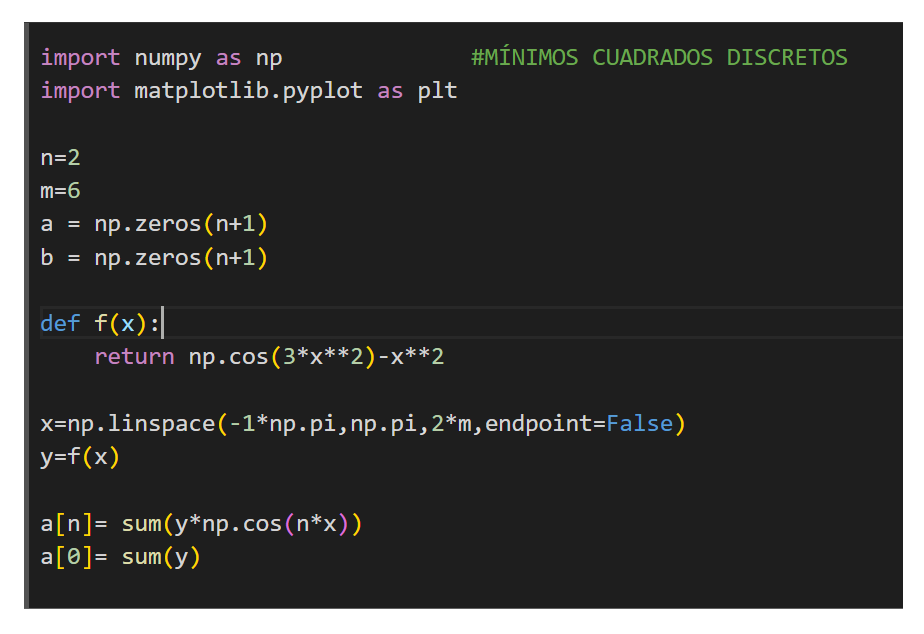
\includegraphics[width=.85\paperwidth]{p7-code1.png}
        \caption*{}
    \end{figure}
\end{frame}

\begin{frame}{Implementación}
    \begin{figure}
        \centering
        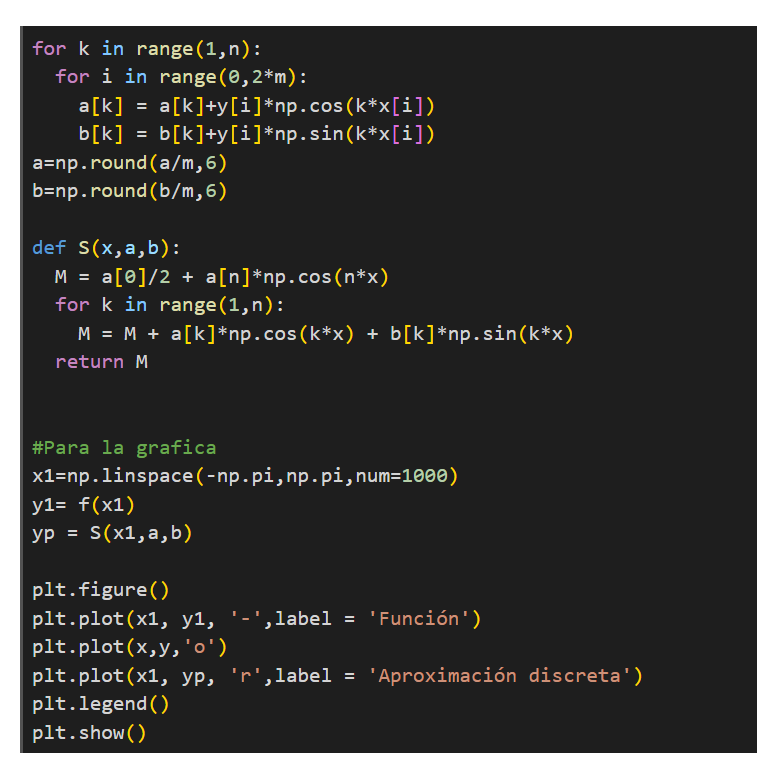
\includegraphics[width=.58\paperwidth]{p7-code2.png}
        \caption*{}
    \end{figure}
\end{frame}

\begin{frame}{Resultados}
    \begin{figure}
        \centering
        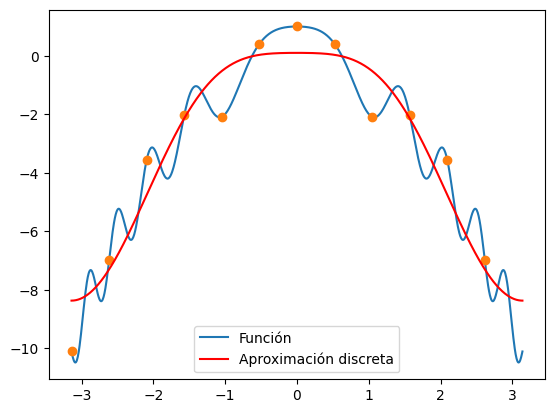
\includegraphics[width=.75\paperwidth]{p7-Aprox-discreta.png}
        \caption{Para $n=2$ y $m=6$}
    \end{figure}
\end{frame}

\begin{frame}{Results}
    \begin{figure}
        \centering
        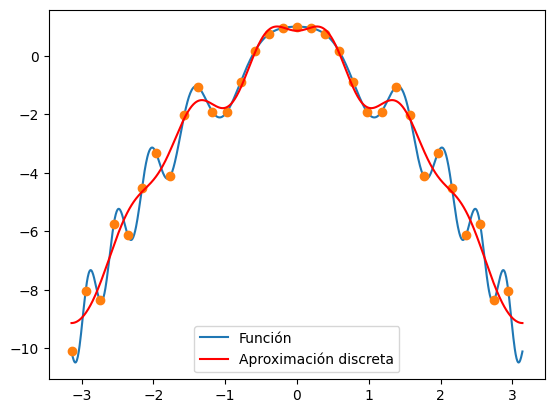
\includegraphics[width=.75\paperwidth]{p7-A-discreta2.png}
        \caption{Para $n=7$ y $m=16$}
    \end{figure}
\end{frame}

\begin{frame}
    \frametitle{Results}

    \begin{figure}
        \centering
        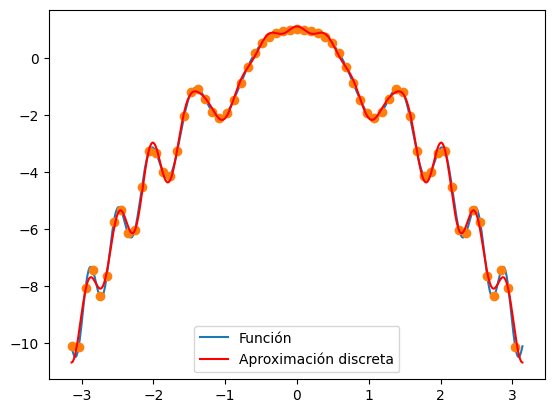
\includegraphics[width=.75\paperwidth]{p7-A-discreta3.png}
        \caption{Para $n=15$ y $m=32$}
    \end{figure}
\end{frame}